%-----------------------------------LICENSE------------------------------------%
%   This file is part of tikz_figures.                                         %
%                                                                              %
%   tikz_figures is free software: you can redistribute it and/or              %
%   modify it it under the terms of the GNU General Public License as          %
%   published by the Free Software Foundation, either version 3 of the         %
%   License, or (at your option) any later version.                            %
%                                                                              %
%   tikz_figures is distributed in the hope that it will be useful,            %
%   but WITHOUT ANY WARRANTY; without even the implied warranty of             %
%   MERCHANTABILITY or FITNESS FOR A PARTICULAR PURPOSE.  See the              %
%   GNU General Public License for more details.                               %
%                                                                              %
%   You should have received a copy of the GNU General Public License along    %
%   with tikz_figures.  If not, see <https://www.gnu.org/licenses/>.           %
%------------------------------------------------------------------------------%

% Use the standalone class for displaying the tikz image on a small PDF.
\documentclass[crop, tikz]{standalone}

% Import the tikz package to use for the drawing.
\usepackage{tikz}

% Tikz packages used.
\usetikzlibrary{arrows.meta, decorations.markings, calc}

% Begin the document.
\begin{document}

    % Draw the figure.
    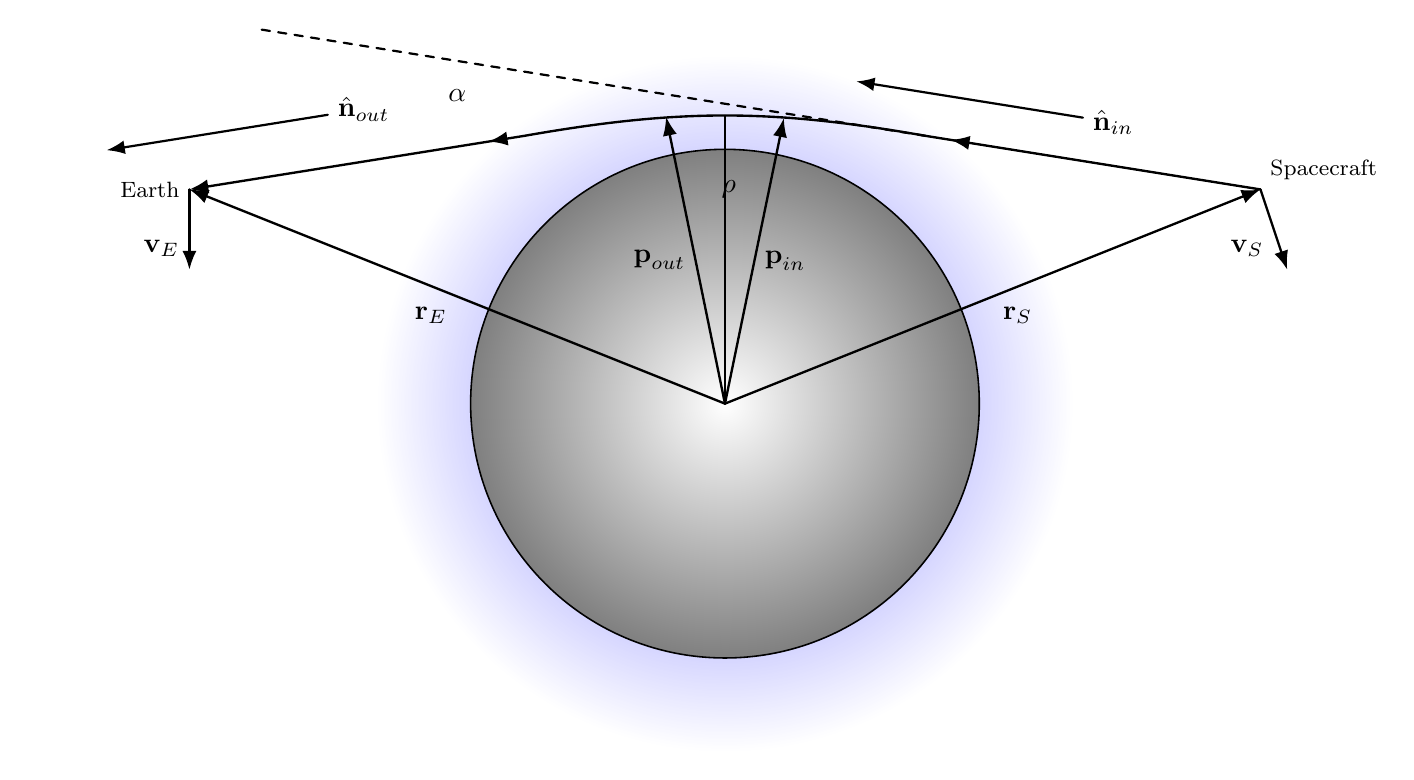
\begin{tikzpicture}[%
        > = Latex,
        line width = 0.2mm,
        line cap = round,
        scale = 1.7
    ]

        % Start a group to locally define variouble for color.
        \begingroup

            % Color for the ring.
            \newcommand{\rcolor}{white!100!blue}

            % Coordinates
            \coordinate (S) at (4.0, 1.6);
            \coordinate (E) at (-4.0, 1.6);
            \coordinate (O) at (0.0, 0.0);
            \coordinate (p1) at (-1.5, 2.0);
            \coordinate (p2) at (1.5, 2.0);
            \coordinate (p_in) at (0.44, 2.133);
            \coordinate (p_out) at (-0.44, 2.144);
            \coordinate (P) at (0.0, 2.2);
            \coordinate (v_S) at (4.2, 1.0);
            \coordinate (v_E) at (-4.0, 1.0);
            \coordinate (dash) at (-3.5, 2.8);

            % Labels for various points.
            \node at (E) [left] {\footnotesize{Earth}};
            \node at (S) [above right] {\footnotesize{Spacecraft}};

            % Draw outer ring to simulate the atmosphere.
            \draw[%
                draw = none,
                inner color = blue,
                outer color = \rcolor,
                opacity = 0.6
            ] (O) circle (26mm) (O) circle (1.9);

            % Draw inner circle.
            \draw[%
                inner color = white,
                outer color = gray
            ] (O) circle (1.9);

            % Draw path for the emitted signal through the atmosphere.
            \begin{scope}[line width = 0.3mm, ->]
                \draw[%
                    postaction = {decorate},
                    decoration = {%
                        markings,
                        mark = at position 0.29 with \arrow{Latex},
                        mark = at position 0.72 with \arrow{Latex}
                    }
                ] (S) to (p2) to[bend right = 10] (p1) to (E);

                \path (O) edge node [right] {$\textbf{p}_{in}$} (p_in);
                \path (O) edge node [left] {$\textbf{p}_{out}$} (p_out);
                \path (O) edge node [below left] {$\mathbf{r}_{E}$} (E);
                \path (O) edge node [below right] {$\mathbf{r}_{S}$} (S);
                \path (S) edge node [below left] {$\mathbf{v}_{S}$} (v_S);
                \path (E) edge node [below left] {$\mathbf{v}_{E}$} (v_E);
            \end{scope}

            % More labels.
            \node (nin) at (2.9, 2.1) {$\hat{\mathbf{n}}_{in}$};
            \node (nout) at (-2.7, 2.2) {$\hat{\mathbf{n}}_{out}$};

            % Draw more lines.
            \begin{scope}[thick]
              \draw[shorten >=1cm,shorten <=0cm,->] (nin) to +($(p2)-(S)$);
              \draw[shorten >=1cm,shorten <=0cm,->] (nout) to +($(E)-(p1)$);
              \draw[dashed] (p2) to (dash);
              \draw (O) to (0.0, 2.15);
            \end{scope}

            % And some more labels.
            \node at (-2.0, 2.3) {$\alpha$};
            \node at (-0.1, 1.6) [right] {$\rho$};
        \endgroup
    \end{tikzpicture}
\end{document}
